%%%%%%%%%%%%%%%%%%%%%%%%%%%%%%%%%%%%%%%%%%%%%%%%%%%%%%%%%%%%%%%%%%%%%%
% LaTeX Template: Curriculum Vitae
%
% Source: http://www.howtotex.com/
% Feel free to distribute this template, but please keep the
% referal to HowToTeX.com.
% Date: July 2011
% 
%%%%%%%%%%%%%%%%%%%%%%%%%%%%%%%%%%%%%%%%%%%%%%%%%%%%%%%%%%%%%%%%%%%%%%
% How to use writeLaTeX: 
%
% You edit the source code here on the left, and the preview on the
% right shows you the result within a few seconds.
%
% Bookmark this page and share the URL with your co-authors. They can
% edit at the same time!
%
% You can upload figures, bibliographies, custom classes and
% styles using the files menu.
%
% If you're new to LaTeX, the wikibook is a great place to start:
% http://en.wikibooks.org/wiki/LaTeX
%
%%%%%%%%%%%%%%%%%%%%%%%%%%%%%%%%%%%%%%%%%%%%%%%%%%%%%%%%%%%%%%%%%%%%%%

%%%%%%%%%%%%%%%%%%%%%%%%%%%%%%%%%%%%%%%%%%%%%%%%%%%%%%%%%%%%%%%%%%%%%%
% Specify the type of the document
% document type alternative: article,report,book and slides
%%%%%%%%%%%%%%%%%%%%%%%%%%%%%%%%%%%%%%%%%%%%%%%%%%%%%%%%%%%%%%%%%%%%%%
\documentclass[paper=a4,fontsize=11pt]{scrartcl} % KOMA-article class

%%% Call macro sets				
\usepackage[english]{babel}

%%% Character Encode
\usepackage[utf8]{inputenc}                   % 替换你正在使用的编码
\usepackage{CJKutf8}

\usepackage[protrusion=true,expansion=true]{microtype}
\usepackage{amsmath,amsfonts,amsthm}     % Math packages
\usepackage{graphicx}                    % Enable pdflatex
\usepackage[svgnames]{xcolor}            % Colors by their 'svgnames'
\usepackage{geometry}
	\textheight=700px                   % Saving trees ;-)
\usepackage{url}
\usepackage{multicol}                    % multiple columns

\frenchspacing                           % Better looking spacings after periods
\pagestyle{empty}                        % No pagenumbers/headers/footers

%%% Custom sectioning (sectsty package)
%%% ------------------------------------------------------------
\usepackage{sectsty}

\sectionfont{%			              % Change font of \section command
	\usefont{OT1}{phv}{b}{n}%		   % bch-b-n: CharterBT-Bold font
	\sectionrule{0pt}{0pt}{-10pt}{3pt}}

%%% Macros
%%% ------------------------------------------------------------
\newlength{\spacebox}
\settowidth{\spacebox}{8888888888}			% Box to align text
\newcommand{\sepspace}{\vspace*{1em}}		% Vertical space macro

\newcommand{\Title}[1]{ % Name
		\begin{center}
			\Huge #1
		\end{center}
		\par \normalsize \normalfont} % \par 换行
		
\newcommand{\Slogan}[1]{ % Slogan (optional)
		\large \usefont{OT1}{phv}{m}{n}\hfill \textit{#1} % \textit italic text
		\par \normalsize \normalfont}

\newcommand{\Section}[1]{\section*{ #1 }}          % * 去掉section标号

\newcommand{\SubSection}[2]{
	\sepspace \noindent \textbf{#1} \hfill      % 项目名称
	\colorbox{Black}{\parbox{7em}{\hfill\color{White}#2}} \par  % 时间
	\normalsize \par \sepspace}


\newcommand{\Personal}[2]{
		\noindent\hangindent=2em\hangafter=0 % Indentation
		\parbox{\spacebox}{#1}     % Box to align text		       
		\hspace{1.5em} #2 \par}    % Entry value

\newcommand{\Education}[3]{
		\noindent \textbf{#1} \hfill      % \textbf 加粗
		\colorbox{Black}{%
		\parbox{7em}{%
		\hfill\color{White}#2}} \par  % Duration
		#3
		\normalsize \par}

\newcommand{\Work}[3]{
		\noindent \textbf{#1} \hfill      % 公司名称
		\colorbox{Black}{\parbox{7em}{\hfill\color{White}#2}} \par  % 时间
		#3 \par              % 职位
		\normalsize \par}

\newcommand{\Academic}[2]{
		\noindent \textbf{#1} \par      % 分类
		\hangindent=2em \small #2 % 成果项
		\normalsize \par}

%%% Begin Document
%%% ------------------------------------------------------------
\begin{document}
\begin{CJK}{UTF8}{gbsn}                       % 详情参阅CJK文件包
% you can upload a photo and include it here...
%\begin{wrapfigure}{l}{0.5\textwidth}
%	\vspace*{-2em}
%		\includegraphics[width=0.15\textwidth]{photo}
%\end{wrapfigure}

\Title{个人简历}
% \MySlogan{RubyChina}

\sepspace % set spacing between lines

%%% Personal details
%%% ------------------------------------------------------------
\Section{基本信息}

\begin{multicols}{2}                           % 分两栏
	\Personal{姓 名}{姜政冬}
	\Personal{电 话}{18668150635}
	\Personal{邮  箱}{\url{xautjzd@gmail.com}}
	\Personal{地  址}{浙江省杭州市}
	\Personal{英 语}{CET-6}

\columnbreak                                   % 强制分栏
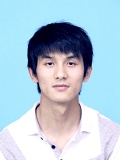
\includegraphics[width=0.2\textwidth\hfill]{xautjzd1.jpg}
\end{multicols}

%%% Education
%%% ------------------------------------------------------------
\Section{教育经历}

\Education{西安理工大学}{2012.09-2015.07}{专业: 软件工程 学历: 硕士(保送)}
\sepspace
\Education{西安理工大学}{2008.08-2012.06}{专业: 网络工程 学历: 学士}

%%% Work
%%% ------------------------------------------------------------
\Section{工作经历}

\Work{杭州端点网络科技有限公司-低代码平台}{2020.07-现在}{高级 Java 开发工程师}
\Work{杭州端点网络科技有限公司-Paas 平台}{2018.07-2020.06}{高级 Golang 开发工程师}
\sepspace
\Work{杭州网易有限网络公司-网易云容器服务}{2015.07-2018.07}{高级 Java 开发工程师}

%%% Project
%%% ------------------------------------------------------------
\Section{项目经历}

\SubSection{端点低代码平台}{2020.07-现在}
项目描述: 端点低代码平台为元数据驱动开发平台,用于支撑端点业务系统,可基于此平台针对标品快速二开,满足企业交付的差异化需求。专注于企业中后台系统,提供了一套研发体系,定义了一套DSL \& 研发框架,可快速构建出业务系统。\par
\sepspace
项目职责:
\begin{itemize}
\item 负责研发框架机制部分功能开发,包括 i18n 机制、机器翻译、元数据发布流程、事件监听机制等
\item 负责后端研发规范制定 \& 落地
\end{itemize}

\SubSection{端点 PaaS 平台}{2018.07-2020.06}
项目描述:端点 PaaS 平台(名为 Dice)实现了源码托管、CI/CD、中间件管理、微服务治理、快数据、运维监控等,有效地提高企业的 IT 研发、
运维、运营效率,降低成本。提供了遵循 GitFlow 规范的代码托管机制,采用 Pipeline 模式实现了代码编译、测试、
打包等一系列的构建流程。遵循基础设施即代码设计理念,实现微服务一键编排部署。通过 pipeline.yml 描述构建流水线,
dice.yml 描述服务部署资源规格与依赖中间件等。底层支持 Kubernetes \& DCOS \& 阿里云 EDAS 等 ,支持 SaaS 化部署与私有化部署两种方式。\par
\sepspace
项目职责:  
\begin{itemize}
\item 负责开发并维护 Dice cli(基于 cobra),将 CI/CD、市场推送等关键能力通过 cli 提供给用户,为用户提效
\item 负责开发并维护 Dice 平台组织结构元数据(企业、项目、应用、runtime、service 等)、集群元数据、ACL 数据、机器 \& 服务实例元信息存储
\item 负责开发并维护 Dice 平台事件管理,包括迭代、需求、任务、缺陷及与 MR 关联等功能
\item 负责开发并维护 Dice 平台版本管理(通过 dice.yml 文件描述应用紧密相关的多个 service \& 所依赖中间件,发布时以 dice.yml 为最小粒度)
\item 参与共建应用市场(自研工作流框架,通过 action 扩展功能,工作流任务通过 pipeline.yml 进行描述,与 github actions 类似),开发了 java-deploy, js deploy 等 action
\item 负责开发并维护 Dice 平台公告、工单等功能
\item 实现了 Flink/Spark 调度器插件(自研调度器支持插件化开发,目前支持 K8s/K8s Job/Marathon/Metronome//Flink/Spark/EDAS)
\end{itemize}

\SubSection{网易云容器服务}{2015.07-2018.07}
项目描述: 网易云容器服务基于 Kubernetes,将 Kubernetes 相关功能产品化提供给用户,包含 Namespace、
无状态工作负载、有状态工作负载、服务发现、事件、云盘挂载等。另外容器服务团队还承担整个网易云控制台开发,
包括各垂直服务接入、API 流控、服务灰度发布等。\par
\sepspace
项目职责: Namespace、无状态工作负载研发;参与网易云私有化部署,负责容器服务、镜像仓库服务裁剪与适配,
去除公有云组件依赖;云主机、云硬盘、弹性公网IP、负责均衡、对象存储、RDS、Redis、日志服务等透明转发;
基于Redis实现流控,防止用户恶意刷API。

\SubSection{网易云镜像仓库}{2015.07-2018.07}
项目描述: 实现与运维网易云镜像仓库服务,包括镜像分类展示、镜像搜索、镜像收藏、镜像构建(包含
Dockerfile 构建与源码构建两种方式)、运行中容器保存为镜像、镜像可用性检查等功能,基于原生
Docker Registry 开发认证授权功能,对接网易认证系统,开发 registry 后端存储插件对接网易对象
存储,将镜像存储于网易对象存储。\par
\sepspace
项目职责: 独自开发与运维网易云镜像仓库

\SubSection{分布式配置管理平台}{2017.05-2018.07}
项目描述:基于 Disconf 搭建分布式配置管理平台,推动容器服务各组件将配置集中托管在配置管理平台,
统一维护。原生 Disconf 无配置 review,为实现此功能,特开发了 git2disconf 服务,将配置集中托管
在git平台,基于 git mr 进行 review,review 完成后通过 disconf API 同步至 Disconf。\par
\sepspace
项目职责: 独自开发与运维配置管理平台,采用容器化部署

%%% Skills
%%% ------------------------------------------------------------
\Section{个人技能}

\begin{itemize}
    \item 熟悉 Java,6年项目使用经验; 熟悉 Golang,2年项目使用经验; 熟悉 shell \& Linux 命令
	\item 熟悉 MySQL/RabbitMQ/Etcd/Redis 等中间件, 了解 Kafka, RocketMQ
	\item 熟悉 Docker、Docker Registry、Kubernetes,了解DCOS、Mesos、Marathon,有阅读 kubernetes 源码经验
	\item 熟悉 dns/http 等协议,阅读过相关 RFC, 利用 tcpdump/wireshark 分析过协议细节
	\item 熟悉 MacOS/Linux 环境 \& 常用命令
	\item 熟练掌握 Git/Vim/Maven/Markdown/Goland/Intellij IDEA 等
    \item 了解Rust, 通过 Rust 官网提供的 Rust book 学习过Rust 语法
	\item 了解 Raft \& Paxos 等分布式一致性协议、分布式相关的 CAP \& BASE 理论
	\item 了解 Tex/VimScript
\end{itemize}

%%% Academic Honors
%%% ------------------------------------------------------------
\Section{学术成果}

\Academic{论文发表}{基于灰色系统理论的气调库环境预测模型[J]. 计算机系统应用,2014,23(3):123-126,118}
\sepspace

\Academic{软件著作权}{气调库环境监测系统,国家版权局,软件登记号:2014SR019840,2014.2.19}
\Academic{}{果品生产经营信息管理系统,国家版权局,软件登记号:2014SR039978,2014.04.09}
\sepspace

%%% Hobby
%%% ------------------------------------------------------------
\Section{兴趣爱好}
热爱羽毛球、游泳、网球等运动,喜欢阅读宏观经济学、历史、地理等书籍

%%% Self Asessment
%%% ------------------------------------------------------------
\Section{自我评价}
热爱编程,专注于服务端;学习能力较强,乐于接受新鲜事物,分析解决问题能力较强
\end{CJK}     % 结束中文环境
\end{document}
